%% Dissertationsvorlage
%%
%% Karlsruhe Institute of Technology
%% Institute for Program Structures and Data Organization
%% Chair for Software Design and Quality (SDQ)
%%
%% Dr.-Ing. Erik Burger
%% burger@kit.edu
%%
%% Siehe https://sdq.kastel.kit.edu/wiki/Dokumentvorlagen

% Für Dokumentoptionen siehe README.md

\documentclass[format=a4-sdq]{sdqdiss}

%% --------------------------------
%% | Font and language setup      |
%% --------------------------------

\usepackage[T1]{fontenc}
\usepackage[utf8]{inputenc} % allow utf-8 input
\usepackage[T2A,T1]{fontenc}  % use 8-bit T1 fonts, T2A Cyrillic fonts

% better looking fonts
\usepackage[tt=false, type1=true]{libertine}
\usepackage{libertinust1math}
% Improves general appearance of the text
\usepackage[protrusion=true,expansion=true,kerning]{microtype}

% set up for Japanese
\usepackage{CJKutf8}
\newcommand{\ja}[1]{\begin{CJK}{UTF8}{min}#1\end{CJK}}

% Für Sprachumschaltung
\usepackage[russian,ngerman,english]{babel}
\selectlanguage{english}

%% --------------------------------
%% | Misc setup                   |
%% --------------------------------

\usepackage{csquotes}

% Abstract
\newcommand{\Abstract}[1][Abstract]{\chapter*{#1}\addcontentsline{toc}{chapter}{#1}\markboth{#1}{#1}} 

%% Nur als Beispiel – im endgültigen Dokument bitte entfernen
\usepackage{blindtext}
% TikZ ist kein Zeichenprogramm
\usepackage{tikz}
% Schöne Tabellen
\usepackage{booktabs}
%% /Beispiel

%% --------------------------------
%% | Heading setup                |
%% --------------------------------

% Fancy chapter headings
\usepackage{quotchap}
% adjustment of header font
\makeatletter
\renewcommand*{\chapnumfont}{%
  \usefont{T1}{\@defaultcnfont}{n}{n}\fontsize{100}{130}\selectfont%
  \color{chaptergrey}%
}
\makeatother
% make headlines use serif font
\addtokomafont{disposition}{\rmfamily}

% % TODO: consider using appendix package (see msc)
% % enable appenix
% \usepackage[toc,page]{appendix}
% \noappendicestocpagenum

%% --------------------------------
%% | Bibliographie setup          |
%% --------------------------------

%% Biber statt BibTeX, siehe README.md
\usepackage[citestyle=numeric,style=numeric,backend=biber]{biblatex}
\addbibresource{bib/dis.bib}

%% --------------------------------
%% | Title page                   |
%% --------------------------------

\title{Final Dissertation Title Which Will Probably Need Multiple Lines}
\author{Tarek Saier}
\subject{}

\subtitle{
\vskip2em
zur Erlangung des akademischen Grades eines\\[1em]
Doktors der Ingenieurwissenschaften\\
(Dr.-Ing.)\\[1em]
von der Fakultät für Wirtschaftswissenschaften\\
des Karlsruher Instituts für Technologie (KIT)\\[1em]
vorgelegte\\
Dissertation\\[1.5em]
von
}

\author{{\LARGE M.\,Sc. Tarek Saier}}

\publishers{%
\flushleft\small
\begin{align*}
    &\text{Tag der mündlichen Prüfung:} &\text{XX. Monat XXXX}\\
    &\text{Referent:} &\text{Prof. Dr. N. N.}\\
    &\text{Korreferent:} &\text{Prof. Dr. M. M.}
\end{align*}
}

\date{}  % used to supress printing a date

%% --------------------------------
%% | Document start               |
%% --------------------------------

\begin{document}
\selectlanguage{ngerman}
\maketitle

%% --------------------------------
%% | Abstract                     |
%% --------------------------------

% Römische Seitenzahlen
\frontmatter

%% Englischer Abstract
\selectlanguage{english}
\Abstract{}
% motivation
Scientific publications are written by humans \emph{for humans}.
However, vital infrastructure in academia relies on the processing of publications \emph{by computers}.
For example, academic search engines and performance indicators, which are indispensable for literature review and decision making, require machine-readable representations of publications.
Bridging the gap from a medium \emph{for humans} to something suitable for processing \emph{by computers} is a challenging and error-prone process.

% gap
Existing methods for the creation of data representing publications, and by extension the data they produce, are limited in various ways. Specifically, there are shortcomings regarding documents' interconnections, language coverage, and content representation granularity. For example, widely used data sets have highly incomplete citation networks, are limited to publications written in English, or fail to accurately capture mathematical notation. As a consequence, applications and research building on this data are of limited scope and validity.

% solution
To address these issues, we present a set of data mining and information extraction approaches that enable the creation of machine-readable publication corpora more complete, extensive, and of finer granularity than previously available. We quantify our contributions to better data quality along the dimensions relevance, accuracy, timeliness, comparability, and completeness, and achieve improvements across all of them.

In particular, we present the following.
As the foundation of our research, we introduce a method for creating a large-scale corpus of linked, full-text documents from publications' \LaTeX\ sources.
Utilizing the resulting corpus, we further present approaches yielding advances in three areas.
First, we demonstrate improvements in the completeness of citation networks though the use of a blocking and matching method, as well as improvements in the granularity of document representations.
Second, we show advances in the language coverage of document interconnections through identifying and analyzing cross-lingual citations.
Third, we present information extraction approaches for fine-granular representations of research artifacts and their parameters.

% summary
Overall, our approaches address key shortcomings of existing methods for the creation of data representing publications.
For each of our approaches, we demonstrate its viability and benefits through evaluations and practical large-scale applications.
Our methods have already been adopted in several parts of the research community, which further confirms their utility.


%% Deutsche Zusammenfassung
\selectlanguage{ngerman}
\Abstract[Zusammenfassung]{}
\Blindtext[10]


%% --------------------------------
%% | ToC                          |
%% --------------------------------

% Sprache der Dissertation
\selectlanguage{english}

\tableofcontents

% Linksbündige Einträge ohne Einzug
\listoffigures
\listoftables

%% --------------------------------
%% | Content                      |
%% --------------------------------

% Arabische Seitenzahlen
\mainmatter

\part{Introduction}
\chapter{Introduction}
\label{chp:introduction}

% What do I want to say and convey here?
% - scientific publications are the ``footprint'' and ``medium of discourse'' of academic progress
% - structured representation

% establish the nature and role of scientific publications
Scientific publications are the \emph{discourse medium} and \emph{literary footprint} of academic progress. As such, they play a vital role in the everyday workings and advancement of academia.
% segue to the digital
Historically, this role manifested itself physically---through ink on paper. In time, digital methods for authoring %/composition?
and distribution enabled more efficient ways of dissemination.
Today, scientific publications are predominantly authored, distributed, consumed, and archived digitally~\cite{Lamers2018}. However, the form of today's digital publications still retains numerous and deep traces of its physical ancestry.

% Digital dissemination makes the transfer of new knowledge into the research community faster and cheaper. Digital archives enable search technology and analytics to operate on our \emph{literary footprint} of past and present academic progress. In this way, digitization facilitates both faster progress in science, \emph{and} technology helping scientists to keep up with the increase in speed. However, today's form of digital publications is far from optimal for powering such technology. In fact, the form of today's digital publications poses significant challenges for 

% While there lies enormous potential in a digital record of science, there remain significant challenges to realizing this potential. A key cause of these challenges is the historical baggage of today's digital publications. This dissertation is in pursuit of tackling these challenges.

% There lies enormous potential in a digital record of science. But realizing this potential

The historical baggage manifesting itself in the PDF files we read, share, and author, poses significant challenges to realizing the full potential of a digital record of science. While digital services in academia such as search and recommendation do exist, they are powered not by publications themselves, but rather by more structured, derivative representations of publications. The same holds for analyses of publications. The creation of such structured representations %/derivates?
is challenging and error prone, leading to a risk of subpar services and erroneous analyses. This dissertation represents and effort to tackle this challenge and alleviate the quality of structured representations of scientific publications.

% (random alliteration: structured surrogates of academic archives)

% - b/c of discrepancy between current form and what would be even better for digital dissemination and use (e.g. more structured), structured derivates of publications that enable digital services are of limited quality
% - historical baggage in part b/c still meant for human consumption
% - gap(?) between “pure” digital form and current form hinders more efficient use in digital services surrounding publications and academia

\section{Motivation}

% What do I want to say and convey here?
% - why do we have/need scholarly data?
% - in contrast to intro paragraphs above, make *necessity* of scholarly data for mitigating information overload clear
% - also make clear why there was realistic potential in approaching the challenge

In the following, we discuss the importance of structured representations of scientific publications---from hereon referred to as ``scholarly data'' for the sake of legibility%
\footnote{Note that in other contexts the term ``scholarly data'' can have a broader meaning than just ``structured representations of scientific publications''. For example, it can also include data on research institutions or funding bodies, without necessitating the context of a publication.}%
---, and based on that derive the motivation of the research project.

Digitization in academia, and with it the inception of scholarly data, has enabled an acceleration of scientific progress. Digital dissemination makes the transfer of new knowledge into the research community faster% as well as cheaper
, and digital archives enable search technology and analytics to operate on large collections of publications. A second factor for acceleration is increased research spending across the world~\cite{CRS2022,OECD2023}. An increase in scientific progress, and with that an increase in the rate at which research results are published, also means a growing challenge for researchers to keep up.

While ...
% * in the olden days there were polymaths
% * nowadays an expert can't humanly keep up with their field
% * → we need assistance
% * → my research in on enabling the creating of such assistance

% * since ever, humans have sought shortcuts
% * in decision making in science: h-imdex etc. (not sure if this fits b/c I don't specifically address such metrics)

% * not only is my research addressing the now pressing and increasing issue of an increasing rate of publication
% * it also tackles blind spots the have been left unaddressed for long (x-ling)



% big picture view on bridging the gap between historical baggage documents (print, scan, PDF, ...) and digital representation
% - large existing current effort
%       - document image dewarping
%       - OCR
%       - PDF based scholarly data stuff


%Measuring the Evolution of a Scientific Field through Citation Frames~~\cite{Jurgens2018} (usable here (or in HyperPIE chapter) for extra justification of focus on parameters of used artifacts)

\begin{infobox-pub}
\textbf{Publication} \fullcite{Saier2020}
\end{infobox-pub}

\begin{infobox-discussion}
\textbf{Discussion} This text should show what a printed text will look like at this place. If you read this text, you will get no information. Really? Is there no information?
\end{infobox-discussion}

\begin{infobox-info}
\textbf{Remark} This text should show what a printed text will look like at this place. If you read this text, you will get no information. Really? Is there no information?
\end{infobox-info}

\begin{infobox-q}
\textbf{RQ1} How can the completeness of the citation network in scholarly data sets be improved?
\end{infobox-q}

\begin{infobox-progress}
      \begin{tabular}{ccl}
        \toprule
        Crit.\tnote{a} & Res.\tnote{b} & Explanation \\
        \midrule
        \textbf{C1} & {\large\textbf{+}} & Representative coverage in physics, mathematics, CS \\
        \textbf{C2} & $\circ$ & Primary focus on text content \\
        \textbf{C3} & {\large\textbf{+}} & $>96$\% accuracy in reference matching \\
        \textbf{C4} & {\large\textbf{+}} & Low noise due to using \LaTeX\ as data source \\
        \textbf{C5} & {\large\textbf{+}} & Publications until end of most recent full year \\
        \textbf{C6} & {\large\textbf{+}} & Provides MAG and arXiv IDs; DOIs in linked MAG \\
        \textbf{C7} & $\circ$ & Not considered at this stage \\
        \textbf{C8} & {\large\textbf{+}} & 42.6\% reference matching success rate \\
        \textbf{C9} & {\large\textbf{+}} & Full-text included \\
        \bottomrule
      \end{tabular}
\end{infobox-progress}

\section{Research Questions}

Research questions are provided as a guidance to the reader, giving a high-level perspective on the insights provided by the publications making up this dissertation.
% RQ "formulas":
% Q: "How can <goal> be achieved? A: "<proposed method>"
% Q: "How can <proposed method aspect> be leveraged to achieve <goal>? A: "<proposed method>"
% Q: "What's the nature of <analysis object>?" A: "<analysis result>

\section{Contributions}

\begin{table}[tb]
\centering
  \caption{Overview of publications reused in this dissertation.}
  \label{tab:primarypublicationoverview}
  \begin{tabular}{cllllclr}
    \hline
    \ & \ & \ & \ & \ & Author & Venue & \ \\
    Chap. & Venue & Year & Type & Length & Position & Rating & Ref. \\
    \hline
    3 & Scientometrics & 2020 & Journal & Full & 1 of 2 & SJR Q1 & \cite{Saier2020} \\
    \arrayrulecolor{lightgrey}\cline{1-8}
    \multirow{2}{*}{4} & JCDL & 2022 & Workshop & Full & 1 of 3 & Core A* & \cite{Saier2022ULITE} \\
    \ & JCDL & 2023 & Conference & Short & 1 of 3 & Core A* & \cite{Saier2023unarXive} \\
    \arrayrulecolor{lightgrey}\cline{1-8}
    \multirow{2}{*}{5} & ICADL & 2020 & Conference & Full & 1 of 2 & Core A & \cite{Saier2020xling} \\
    \ & IJDL & 2022 & Journal & Full & 1 of 3 & SJR Q2 & \cite{Saier2021} \\
    \arrayrulecolor{lightgrey}\cline{1-8}\arrayrulecolor{black}
    6 & ECIR & 2023 & Conference & Full & 1 of 4 & Core A & \cite{Saier2023hyperpie} \\
    \hline
    \end{tabular}
\end{table}

The contributions in this dissertation have been published in peer-reviewed international conferences and journals. Table~\ref{tab:primarypublicationoverview} gives an overview of the publications and the chapters they make up. Venue ranks are taken from Core\refurl{http://portal.core.edu.au/conf-ranks/}{2023-10-12} in the case of conferences and from SJR\refurl{https://www.scimagojr.com/}{2023-10-12} in the case of journals.\footnote{The ranks shown are the rating for the respective publication year, or the most up-to-date ranking if the latter is not listed. For workshops, the rank of the conference at which the workshop is hosted is shown.} For each of the publications, detailed author contributions according to the Contributor Roles Taxonomy\refurl{https://credit.niso.org/}{2023-10-12} are listed at the end of the respective section.

\begin{table}[tb]
\centering
  \caption{Overview of secondary publications not reused in this dissertation.}
  \label{tab:secondarypublicationoverview}
  \begin{tabular}{llllclr}
    \hline
    \ & \ & \ & \ & Author & Venue & \ \\
    Venue & Year & Type & Length & Position & Rating & Ref. \\
    \hline
    ECIR & 2019 & Workshop & Full & 1 of 2 & Core A & \cite{Saier2019} \\
    ECIR & 2020 & Conference & Full & 1 of 3 & Core A & \cite{Saier2020a} \\
    NAACL & 2021 & Workshop & Short & 3 of 4 & Core A & \cite{Krause2021} \\
    AAAI & 2022 & Workshop & Full & 2 of 3 & Core A* & \cite{Shapiro2022} \\
    ECIR & 2022 & Workshop & Full & 4 of 5 & Core A & \cite{Faerber2022bir} \\
    JCDL & 2022 & Conference & Full & 3 of 3 & Core A* & \cite{Nishioka2022} \\
    JCDL & 2023 & Conference & Short & 1 of 3 & Core A* & \cite{Saier2023cocon} \\
    \hline
    \end{tabular}
\end{table}

Additional publications (co-)authored leading up to and during the research period which are not a direct part of this dissertation, but nevertheless informed the overall research trajectory, are listed in Table~\ref{tab:secondarypublicationoverview}. Especially \cite{Saier2019} and \cite{Krause2021}, which constitute the results of the master's thesis preceding the doctoral research period, paved the way for this dissertation.

\section{Outline}
\Blindtext[1]

% unarXive
% |  |  |
% |  |  v
% |  |  blocking
% |  v
% |  unarXive22
% v       |
% xling   v
% |      Hyperpie
% v
% xling+


\part{Contents}
\chapter{Approach}
\section{Description}
\Blindtext
\begin{figure}
\centering
\begin{tikzpicture}
\node[draw] (one) {42};
\draw (one) edge [loop above] (one);
\end{tikzpicture}
\caption{A Figure with long long long long long long long long long long long
long long long long long long long long long long long text}
\label{fig:one}
\end{figure}


%% 
%% Mit Komascript können unterschiedliche Titel für Abschnittsüberschrift,
%% Seitenkopf und Inhaltsverzeichnis gesetzt werden 
%%
\section[tocentry={Text with table (TOC entry)},%
head={Text with table (page head)}]%
{Text with table (section heading)}
\Blindtext

\begin{table}
\centering
% Schöne Tabellen mit Booktabs
\begin{tabular}{rl}
\toprule
\textbf{a header} & \textbf{a header}\\
\midrule
something & important\\
something & important\\
\bottomrule
\end{tabular}
\caption{A Table}
\label{tab:one}
\end{table}

\section{Text with Formulae}
\blindmathpaper[8]


%% Add entry to the table of contents for the bibliography
\printbibliography[heading=bibintoc]

%% --------------------------------
%% | Appendix                     |
%% --------------------------------
\appendix
\chapter{Appendix}

\section{Geographic origin of all cited non-English languages}\label{app:geo_origin}

In Figure~\ref{fig:geo_full} we show the geographic origin of cross-lingual citations in relative terms per cited language (i.e., the numbers of each \emph{row} add up to 1). The distinct diagonal of the matrix and the horizontal line for affiliations in English speaking countries reflect the fact that most cross-lingual citations are either to a local language or originate from an English speaking country. Among cited languages with a low number of total occurrences we can furthermore see a few cases showing unusual distributions, such as a single citation to Macedonian from an author affiliated with a Polish institution, or citations to Icelandic, where a single one originates from Iceland, while the remaining nine originate from institutions in countries where Japanese (3), Italian (1), and Swedish (5) are the most common language.

\begin{figure*}[tb]
\centering
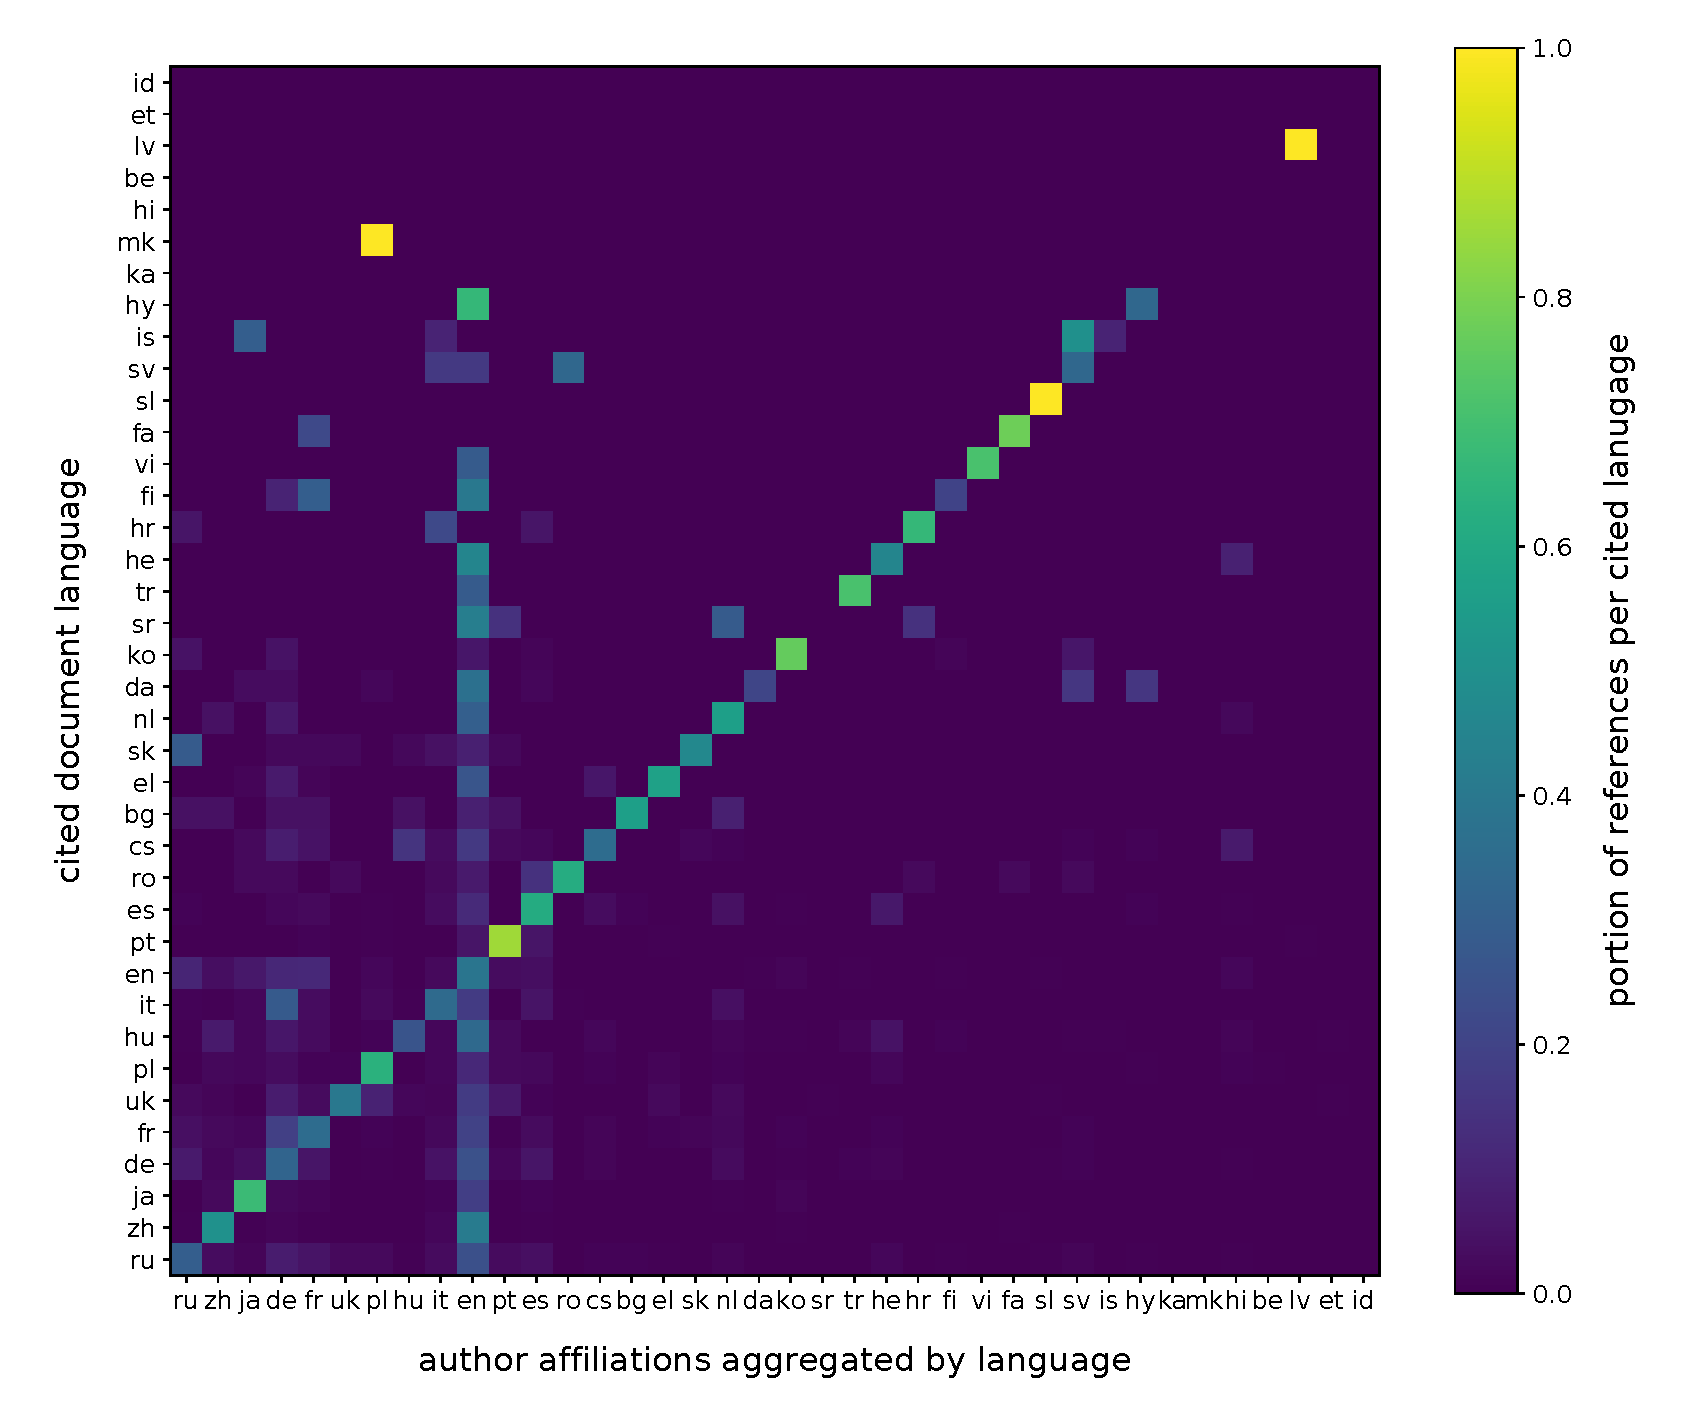
\includegraphics[width=\textwidth]{figures/ref_xling/citlang_to_author_aff_all_relative_crop.pdf}
\caption{Geographic origin of cross-lingual citations (relative count).} \label{fig:geo_full}
\end{figure*}

\section{Citation Intent and Sentiment Classification}\label{app:classifcation}

For the model training of both citation intent classification and citation sentiment classification, we fine-tune SciBERT uncased\footnote{See \url{https://huggingface.co/allenai/scibert_scivocab_uncased}.} using the following model configuration shown in Table~\ref{tab:modelconf}.

\begin{table}
\caption{Model configuration used for training}
 \label{tab:modelconf}
  \centering
  \begin{small}
 \begin{threeparttable}
 \begin{tabular}{lr}
 \toprule
   Hyperparameter & value \\
   \midrule
  attention\_probs\_dropout\_prob &  0.1 \\
  gradient\_checkpointing &  false \\
  hidden\_act &  gelu \\
  hidden\_dropout\_prob &  0.1 \\
  hidden\_size &  768 \\
  initializer\_range &  0.02 \\
  intermediate\_size &  3072 \\
  layer\_norm\_eps &  1e-12 \\
  max\_position\_embeddings &  512 \\
  model\_type &  bert \\
  num\_attention\_heads &  12 \\
  num\_hidden\_layers &  12 \\
  pad\_token\_id &  0 \\
  position\_embedding\_type &  absolute \\
  transformers\_version &  4.4.2 \\
  type\_vocab\_size &  2 \\
  use\_cache &  true \\
  vocab\_size &  31090 \\
   \bottomrule
 \end{tabular}
\end{threeparttable}
  \end{small}
\end{table}

For determining the citation intent, we use the train, validation, and test split provided by the SciCite data set\footnote{See \url{https://huggingface.co/datasets/scicite}.} (train: 74\%, val: 8.3\%, test: 16.9\%). For citation sentiment, we split the Athar data set into train, validation, and test sets into 80\%, 10\%, and 10\%, respectively.



\section{HyperPIE Implementation Details}\label{app:hyperpie-implementation-details}

\paragraph{Fine-Tuned Models:}
We obtain the source code of PL-Marker from the author's GitHub repository\footnote{See \url{https://github.com/thunlp/PL-Marker/}.}. To make it work with our entity and relation schema, we extended the source code in \texttt{run\_acener.py} and \texttt{run\_re.py}. A patch file with all changes is provided in our code share. Our own RE model is a FFNN implemented with 4 hidden layers, each with ReLU activation and dimensions 300, 100, 25 and 2 respectively. All fine-tuned models are trained and evaluated on a local server with a GeForce RTX 3090 (24\,GB).

%  % MLPClassifier(
%  % hidden_layer_sizes=(300, 100, 25, 2),
%  % activation='relu',
%  % solver='adam',
%  % learning_rate_init=0.001,
%  % max_iter=90,
%  % random_state=1,
%  % shuffle=True,
%  % verbose=verbose

\paragraph{LLMs:}
GPT-3.5 was accessed through the official API. The total usage cost for all testing, prompt tuning, and the full evaluation runs sums up to 60\,USD. In zero-shot setting, all open models are run on a high performance compute cluster using the API layer Basaran.\footnote{See \url{https://github.com/hyperonym/basaran/}.} Vicuna and WizardLM  are run on nodes with $4\times$ NVIDIA Tesla V100 (32\,GB). GALACTICA and Falcon are run with half precision on nodes with $4\times$ NVIDIA A100 (80\,GB).

A zero-shot prompt example is shown in Listing~\ref{lst:promptexample}.

\begin{lstlisting}[language=plain,caption=Prompt example.,label=lst:promptexample,breaklines=true,captionpos=b,frame=single,showlines=true,basicstyle=\tiny\ttfamily]
In the context of machine learning and related fields, what (if any) are the entities (datasets, models, methods, loss functions, regularization techniques) mentioned in the LaTeX Input Text below? What (if any) are their parameters and values?

[LaTeX Input Text start]
We use AdamW with a learning rate ($\alpha$) of 1e-3 for /* [...] */
[LaTeX Input Text end]

Answer in the following YAML format.

Format:
---
text_contains_entities: true/false
entities:
  - entity<N>:
      id: e<N>
      name: "<entity name>"
      type: dataset/model/method/loss function/regularization technique
      has_parameters: true/false
      parameters:
        - parameter<M>:
            id: p<N.M>
/* [...] */
...

Only include entities that are of type dataset, model, method, loss function, or regularization technique. Do not output entities that are of another type. Do not include entities of type task, metric, library, software, or API.
Only produce output in the YAML format specified above. Output no additional text.

Output:
\end{lstlisting}

For few-shot prompting, we employed 4\,bit quantization and used the \texttt{llama-cpp-python}\footnote{See \url{https://github.com/abetlen/llama-cpp-python/}.} API. % based on \texttt{llama.cpp}\footnote{See \url{https://github.com/ggerganov/llama.cpp/}.} backend with CUDA multi-GPU acceleration.
We use the default generation setup in \texttt{llama.cpp}
with parameters: temperature = 0, half precision = enabled, and repetition penalty = 1.1. A few-shot prompt example is shown in Listing~\ref{lst:fewshotprompt}.

\begin{lstlisting}[language=plain,caption=Prompt example.,label=lst:fewshotprompt,breaklines=true,captionpos=b,frame=single,showlines=true,basicstyle=\tiny\ttfamily]
### Instruction:
In the context of machine learning and related fields, what (if any) are the entities (datasets, models, methods, loss functions, regularization techniques) mentioned in the LaTeX Input Text below? What (if any) are their parameters and values?

Answer in the following YAML format.

Format:
```
has_entities: true/false
entities:
  - entity<N>:
      id: e<N>
      name: "<entity name>"
      type: dataset/model/method/loss function/regularization technique
      has_parameters: true/false
      parameters:
        - parameter<M>:
            id: p<N.M>
/* [...] */
```

Here are several examples.

### Example 1:

[LaTeX Input Text start]
We use AdamW with a learning rate ($\alpha$) of 1e-3 for /* [...] */
[LaTeX Input Text end]

### Response 1:
```
has_entities: true
  - entity1:
  	  id: e1
      name: "AdamW"
      has_parameters: true
      parameters:
        - parameter1:
            id: p1
/* [...] */
```

### Example 2:

[LaTeX Input Text start]
/* [...] */
[LaTeX Input Text end]

### Response 2:
```
/* [...] */
```

### Example 3:

[LaTeX Input Text start]
/* [...] */
[LaTeX Input Text end]

### Response 3:
```
/* [...] */
```

Only include entities that are of type dataset, model, method, loss function, or regularization technique. Do not output entities that are of another type. Do not include entities of type task, metric, library, software, or API.
Only produce output in the YAML format specified above. Output no additional text.

[LaTeX Input Text start]
We use AdamW with a learning rate ($\alpha$) of 1e-3 for /* [...] */
[LaTeX Input Text end]

### Response:
```
\end{lstlisting}

In the examples given in the few-shot prompts, we omitted the field \texttt{type: dataset/\allowbreak model/\allowbreak method/\allowbreak loss function/\allowbreak regularization technique}, because this information is not part of the gold annotation. As a consequence, the model outputs also tend to skip this attribute.

% \chapter{Bappendix}

% \section{Bar}
% \Blindtext


\end{document}
